\documentclass[aps,prb,twocolumn,superscriptaddress,floatfix,longbibliography, nofootinbib]{revtex4-2}

\usepackage{amsmath,amssymb} % math symbols
\usepackage{bm} % bold math font
\usepackage{graphicx} % for figures
\graphicspath{ {./images/} }
\usepackage{comment} % allows block comments
%\usepackage{ulem} % allows strikeout text, e.g. \sout{text}

\usepackage{minted} % allows colored code
\usepackage{textcomp} % This package gives the text quote '

\usepackage{enumitem}
\setlist{noitemsep,leftmargin=*,topsep=0pt,parsep=0pt}

\usepackage{xcolor} % \textcolor{red}{text} will be red for notes
\definecolor{lightgray}{gray}{0.6}
\definecolor{medgray}{gray}{0.4}

\usepackage{hyperref}
\hypersetup{
colorlinks=true,
urlcolor= blue,
citecolor=blue,
linkcolor= blue,
% bookmarks=true,
% bookmarksopen=false,
}

% Code to add paragraph numbers and titles
\newif\ifptitle
\newif\ifpnumber
\newcounter{para}
\newcommand\ptitle[1]{\par\refstepcounter{para}
{\ifpnumber{\noindent\textcolor{lightgray}{\textbf{\thepara}}\indent}\fi}
{\ifptitle{\textbf{[{#1}]}}\fi}}
\ptitletrue  % comment this line to hide paragraph titles
% \pnumbertrue  % comment this line to hide paragraph numbers

% minimum font size for figures
\newcommand{\minfont}{6}

% Uncomment this line if you prefer your vectors to appear as bold letters.
% By default they will appear with arrows over them.
% \renewcommand{\vec}[1]{\bm{#1}}

% Allows to rewrite the same title in the supplement
\newcommand{\mytitle}{\Huge Face Unlock}

\begin{document}

\title{\mytitle}

\author{
Muhammed Abdullah Shaikh, Khurshed Fitter, Shital Chiddarwar\\
abd@students.vnit.ac.in, khurshedpf@gmail.com, shitalsc@mec.vnit.ac.in\\
\textit{Visvesvaraya National Institute of Technology, Nagpur, India}
}

% \date{}

\begin{abstract}
This is our project report that aims to understand and develop a face recognition framework. We used MNIST, AT\&T and Labelled Faces in the Wild (LFW) datasets during this project. We performed experiment tracking, hyperparameter tuning, and sweeps throughout our work using WandB.\\ Source files are available at: \url{https://github.com/ABD-01/Face-Unlock}.
\end{abstract}

\maketitle
\section{\label{sec:Start}Problem and Motivation}

Face Recognition is a computer vision task that has been extensively studied for several decades. This project was developed at IvLabs\footnote{\url{https://www.ivlabs.in/}}, the AI and Robotics Lab of VNIT, Nagpur. The motivation was to learn and understand the working of face recognition algorithms and \textit{one-shot} learning. Next, we decided to develop the framework for ourselves from scratch and further deploy it on hardware for a face-recognition-based door-lock system.

\section{\label{sec:oneshot}One-Shot Learning}
% \vspace{-4mm}
One-shot learning is a classification task where one example (or a very small number of examples) is given for each class, which is used to prepare a model, that in turn must make predictions about many unknown examples in the future.

This characterizes tasks seen in the field of face recognition, such as face identification and face verification, where people must be classified correctly with different facial expressions, lighting conditions, accessories, and hairstyles given one or a few template photos.

Modern face recognition systems approach the problem of one-shot learning via face recognition by learning a rich low-dimensional feature representation, called face embedding, that can be calculated for faces easily and compared for verification and identification tasks.

Historically, embeddings were learned for one-shot learning problems using a Siamese network. The training of Siamese networks with comparative loss functions resulted in better performance, later leading to the triplet loss function used in the FaceNet system by Google that achieved then state-of-the-art results on benchmark face recognition tasks.

\section{\label{sec:Model}Model Architechture}
% \vspace{-4mm}
\ptitle{ResNet} We use residual neural networks from \textcite{7780459} for this work, mostly ResNet18, but also experimented with ResNet26 and ResNet50. With ResNets, the gradients can flow directly through the skip connections backward from later layers to initial filters.
% insert residual figure

\ptitle{Siamese Network} A Siamese Neural Network \cite{NIPS1993_288cc0ff} is a class of neural network architectures that contain two or more identical subnetworks. ‘identical’ here means, they have the same configuration with the same parameters and weights. Parameter updating is mirrored across both sub-networks. It is used to find the similarity of the inputs by comparing their feature vectors, so these networks are used in many applications.

\ptitle{Triplet Loss} Triplet loss was introduced in \textcite{Schroff_2015}
The loss function penalizes the model such that the distance between the matching examples is reduced and the distance between the non-matching examples is increased. Let $d(x,y) : \mathbb{R}^D \times \mathbb{R}^D \rightarrow \mathbb{R}$ be a distance function in embedding space of dimension $D$. The loss function is defined as:
\begin{equation}
L = \sum_{\substack{a,p,n \\ y_a = y_p \neq y_n}} [d(x_a, x_p) - d(x_a, x_n) + \alpha]_+
\label{eqn:tripletloss}
\end{equation}
 This loss makes sure that, the projection of an anchor point $x_a$, and it's corresponding positive point $x_p$ belonging to the same class (person) $y_a$ is closer than the projection of a negative point $x_n$ belonging to another class $y_n$, by at least a margin $\alpha$.

 \begin{figure}[h]
    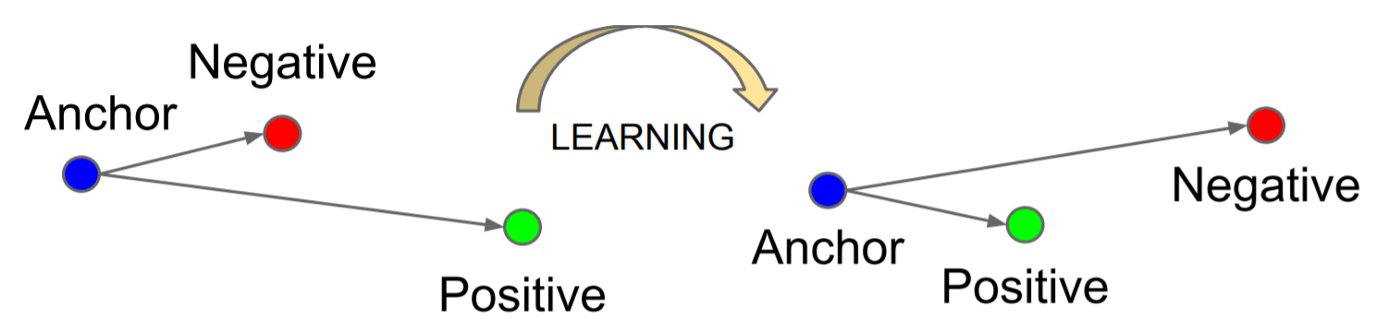
\includegraphics[clip=true,width=\columnwidth]{Tripletloss.png}
    \caption{Triplet Loss} 
     \label{fig:tripletloss}
\end{figure}

\begin{table*}[t]
    \centering
    \begin{center}
    \caption{Result on MNIST Dataset}
    \label{tab:mnsit}
    \begin{tabular}{l|cccccccccc}
    \hline
    \textbf{Class}    & 0       & 1       & 2       & 3       & 4       & 5       & 6       & 7       & 8       & 9       \\
    \hline \hline
    \textbf{Correct}  & 5804    & 6648    & 5830    & 5877    & 5830    & 5274    & 5908    & 5589    & 5777    & 5849    \\
    \textbf{Total}    & 5923    & 6742    & 5958    & 6131    & 5842    & 5421    & 5918    & 6265    & 5851    & 5949    \\
    \textbf{Accuracy} & 97.99\% & 98.60\% & 97.85\% & 95.85\% & 99.79\% & 97.28\% & 99.83\% & 89.20\% & 98.73\% & 98.31\%\\
    \hline
    \end{tabular}
    \end{center}
\end{table*}

\section{\label{sec:Experiments}Experiments}
\section{\label{sec:MNIST}MNIST}
Implemented as a warmup for the project to gain an understanding of one-shot learning and siamese nets.
The model was trained only on 100 images of classes 0,1,2. Images of rest classes i.e 3-9 were kept hidden during the training phase.
The evaluation was done on a 10-way 1-shot basis, wherein the support set Fig. \ref{fig:support} had only one sample from each class 0 to 9.

\begin{figure}[h]
    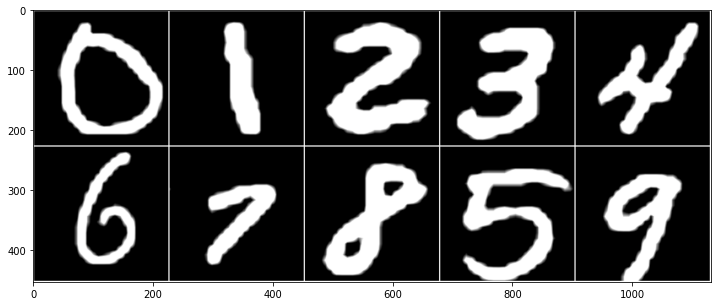
\includegraphics[clip=true,width=\columnwidth]{support.png}
    \caption{Support Set for MNIST one-shot task.} 
     \label{fig:support}
\end{figure}


\section{\label{sec:ATT}AT$\&$T Face Dataset}
% \vspace{-5mm}
\ptitle{Dataset Information}
The AT$\&$T face dataset, “(formerly ‘The ORL Database of Faces’), contains a set of face images taken between April 1992 and April 1994 at AT&T Laboratories Cambridge. It contains 10 different images of 40 distinct people with 400 face images. The database was used in the context of a face recognition project carried out in collaboration with the Speech, Vision and Robotics Group of the Cambridge University Engineering Department.

Besides the fact that the images have the same background and same size, the images were converted to gray level and pixel values were scaled from 0 to 1.

\ptitle{Offline Triplet Mining}
In this approach, we first generate the triplets manually and then fit the data to the network. We used two different types of methods
\begin{raggedright}
\begin{enumerate}
    \item All possible triplets - For each image in the dataset (anchor), we choose all possible combinations to make a positive pair, and for each pair choose all possible combination from the remaining class as Negative.
    \item Random triplets - For each image in data (Anchor), randomly sample a Positive image from its class.  Then from each of the other classes sample one image (randomly) as the Negative. Hence, for every Anchor you will have 1 randomly selected positive from it's class and randomly selected Negative from each of the n-1 classes where n is total number of classes.  For every anchor image you would have n-1 triplets. So if you're having 3 classes of 10 images each then you would have 60 triplets
\end{enumerate}
\end{raggedright}
 However this method being too expensive in terms of memory and computation, it was not performed on datasets other than MNIST.

\ptitle{Online Triplet Mining} 
% \vspace{-5mm}
In this approach, we feed a batch of training data, generate triplets using all examples in the batch, and calculate the loss on it. This approach allows us to randomize the triplets and increase the chance to find triplets with high losses. This will help train the model faster. 
\begin{figure}[h!]
    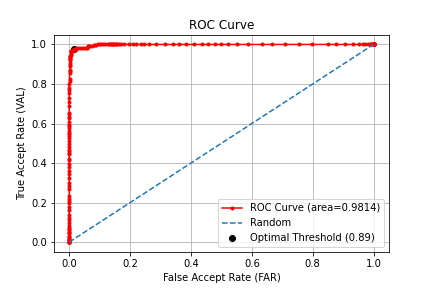
\includegraphics[clip=true,width=\columnwidth]{ROC_curve_ATT_test_dataset.png}
    \caption{An ROC curve is a graph showing the performance of a classification model at all classification thresholds. This curve plots two parameters: (i) True Acceptance Rate, (ii) False Acceptance Rate. The area under ROC curve (AUC) provides an aggregate measure of performance across all possible classification thresholds. AUC = $0.981$} 
     \label{fig:eer_roc}
\end{figure}

\begin{table*}[t]
    \begin{center}
    \caption{Result AT\&T Dataset. $^\dagger$ represents results using online triplet mining, while the rest are using offline mining.}
    \label{tab:att}
    \begin{tabular}{l|c|c|c|c|c}
    \hline
    \textbf{Architechture} & \textbf{No. of learnable parameters} & \textbf{Epochs} & \textbf{Learning Rate} & \textbf{Train Accuracy} & \textbf{Test Accuracy} \\
    \hline \hline
    Plain CNN     & 4,170,400                   & 16     & $0.001$         & 92.67\%        & 88.00\%       \\
    ResNet-18     & 11,235,904                  & 8      & $0.002$         & 99.62\%        & 94.73\%       \\
    ResNet-26     & 17,728,064                  & 20     & $0.002$         & 93.00\%        & 69.00\%       \\
    {ResNet-18}$^\dagger$     & 11,235,904                  & 200    & $0.0002$          & 100\%          & 98.4\%   \\
    \hline
    \end{tabular}
    \end{center}
\end{table*}

\ptitle{Outcome}
During this experiment, the batch size is 100, the face embedding dimension is 64 and the optimizer used was Adam. The results on this dataset are shown in Table \ref{tab:att}. We also studied the Regional Optical Characteristics (ROC) Fig. \ref{fig:eer_roc} and Equal Error Rate (EER) Fig. \ref{fig:eer_att} curves for this setting. We further plotted t-SNE chart of the face embeddings to see the clustering behavior of the model shown in Fig. \ref{fig:tsne_att}.

\begin{figure*}[t!]
    \begin{minipage}[b]{0.45\linewidth}
    \centering
    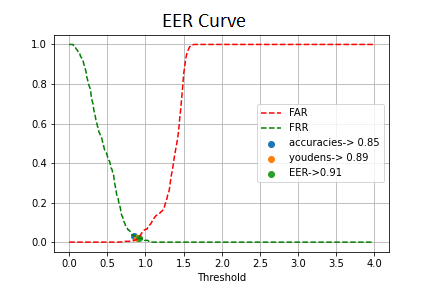
\includegraphics[clip=true,width=1.1\textwidth, height=6cm]{EER_ATT_testdataset.png}
    \caption{The EER is the location on a ROC curve where the false acceptance rate (FAR) and false rejection rate (FRR) are equal. In general, the lower the equal error rate value, the higher the accuracy of the biometric system.}
     \label{fig:eer_att}
     \end{minipage}
     \hspace{0.5cm}
    \begin{minipage}[b]{0.45\linewidth}
    \centering
    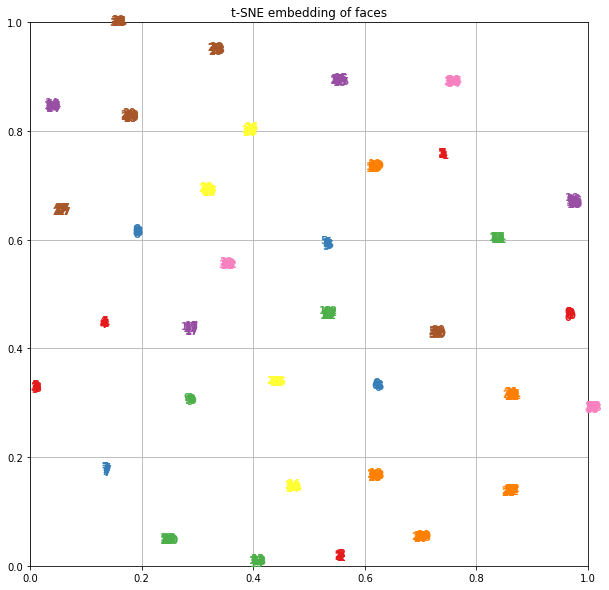
\includegraphics[clip=true,width=\textwidth]{tSNE_embds_ATT_train.png}
    \caption{t-SNE plot for AT\&T dataset.}
    \label{fig:tsne_att}
    \end{minipage}
\end{figure*}

\section{\label{sec:LFW}Labelled Faces in the Wild (LFW)}
\ptitle{Dataset Information} Labeled Faces in the Wild \cite{LFWTech} is a public benchmark for face verification, also known as pair matching. The data set contains more than 13,000 images of faces collected from the web. Each face has been labeled with the name of the person pictured. 1680 of the people pictured have two or more distinct photos in the data set. The only constraint on these faces is that they were detected by the Viola-Jones face detector. Deep Funneled set of LFW images was used for training and evaluation purpose.

\ptitle{Hyperparameter Sweeps} Hyperparameter search or tuning, or optimization is the task of finding the best hyperparameters for a learning algorithm. Hyperparameter sweeps, enable finding the best possible combinations of hyperparameter values for a specific setting by orchestrating a Run and managing experiments for the configuration of our training.  code. We performed a thorough random search for these hyperparameters using WandB \cite{wandb}.

\begin{table}[h!]
    \begin{center}
    \caption{Search on model hyperparameters}
    \label{tab:sweep}
    \begin{tabular}{l|c|c}
    \hline
    \textbf{Hyperparameter}                                        & \textbf{\begin{tabular}[c]{@{}l@{}}Range of\\  Search\end{tabular}} & \textbf{\begin{tabular}[c]{@{}l@{}}Selected \\ Value\end{tabular}} \\
    \hline \hline
    Batch Size                                                     & 40,100                                                     & 256                                                       \\
    Epochs                                                         & 10,50,100,200                                              & 200                                                       \\
    \begin{tabular}[c]{@{}l@{}}Learning\\ Rate\end{tabular}        & 0.002, 0.001, 0.0002, 0.0001                               & 0.002                                                     \\
    \begin{tabular}[c]{@{}l@{}}Embedding \\ Dimension\end{tabular} & 64, 128, 256                                               & 128  \\
    \hline
    \end{tabular}
    \end{center}
\end{table}

\begin{figure*}[t]
    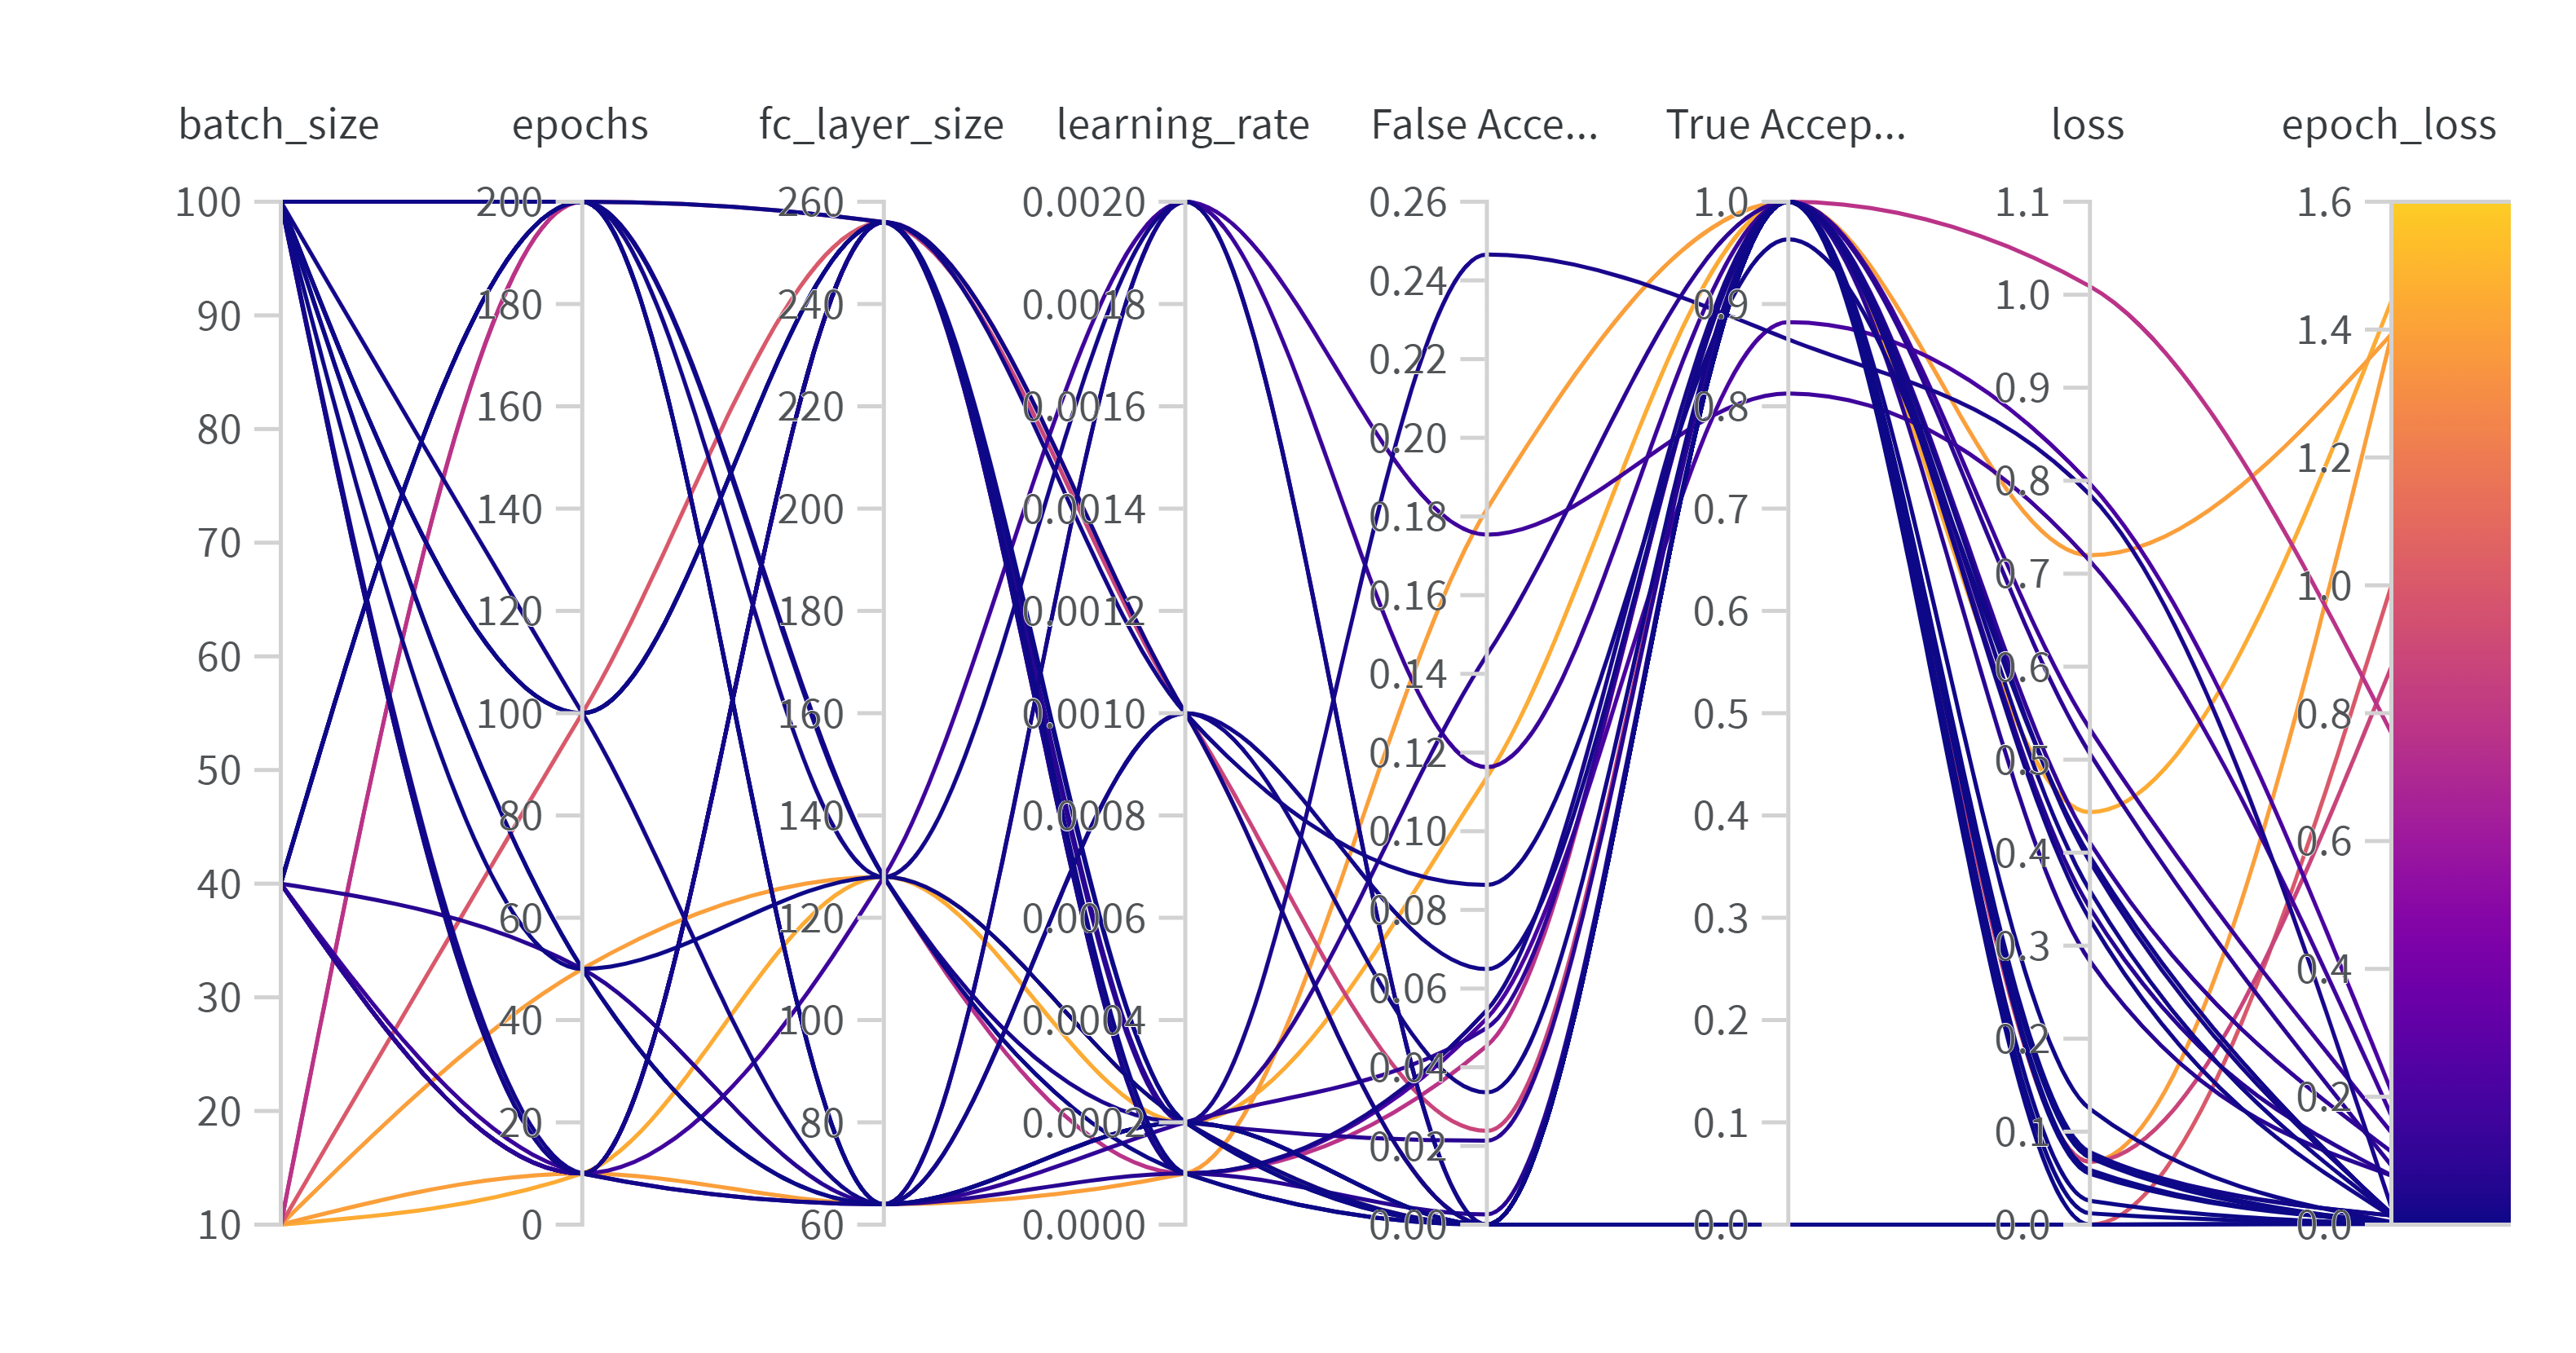
\includegraphics[clip=true,width=2\columnwidth]{face_unlock sweep.png}
    \caption{Hyperparameter Sweep using WandB} 
     \label{fig:sweep}
\end{figure*}

\begin{figure}[h]
    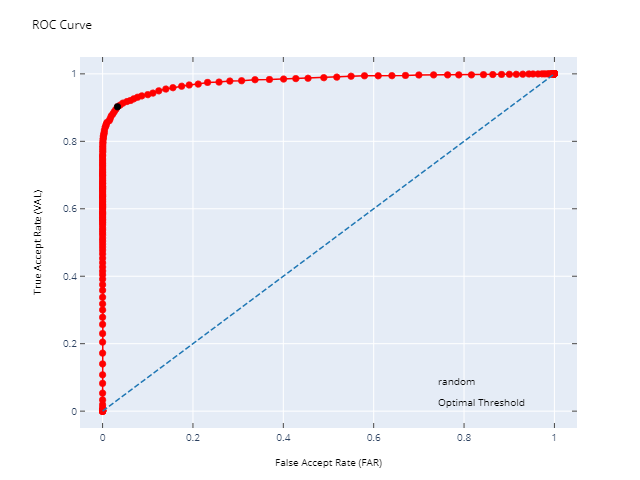
\includegraphics[clip=true,width=\columnwidth]{roc.png}
    \caption{ROC Curve. The Optimal threshold is found to be $1.10$ at TAR=0.864, FAR=0.133. TAR$@$FAR=0.01 is found to be $0.5963$} 
     \label{fig:roclfw}
\end{figure}

\ptitle{Outcome} We use the ResNet-18 \cite{7780459} architecture and the pre-trained weights. We discard the last layer and add a fully connected layer of size 128 corresponding to the embedding dimension. The optimizer used was Adam with a weight decay of 0.01 and rest hyperparameters as mentioned in \ref{tab:sweep}. We start with a learning
rate of $2\times10^{-3}$, and divide it by 2 at every 50 epochs, the chance in learning rate is depicted in Fig. \ref{fig:lr}. We train with batch hard triplet loss as shown in \textcite{tripletmining}. We evaluate our performance referring to \textcite{tamerfacenet} on benchmark for comparison, a 10-fold cross-validation split provided on the official website of LFW. Apart from accuracy, we also studied TAR, FAR, and precision of the model.

\begin{figure*}[t!]
    \begin{minipage}[b]{0.45\linewidth}
    \centering
    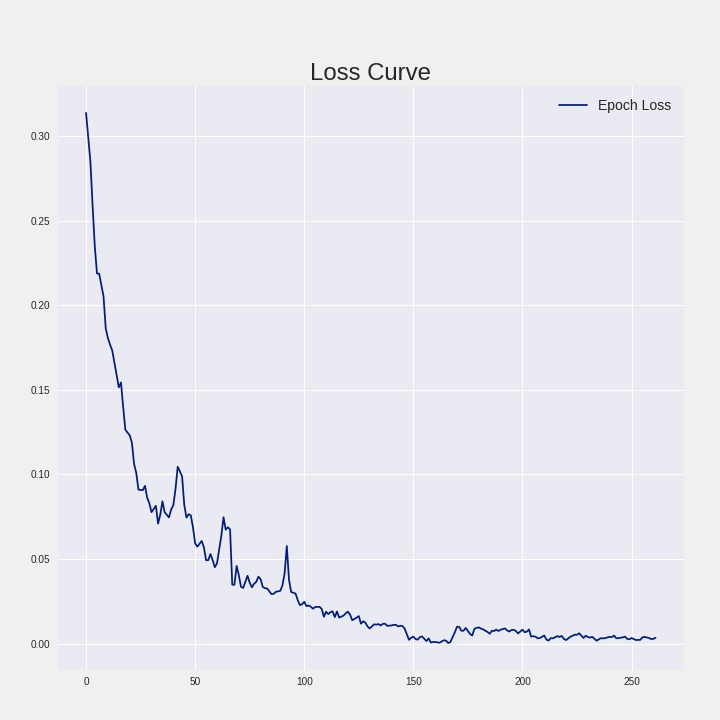
\includegraphics[clip=true,width=1.1\textwidth, height=6cm]{LFWfinal_epochloss.jpeg}
    \caption{Epoch Loss}
     \label{fig:epoch_loss}
     \end{minipage}
     \hspace{1cm}
    \begin{minipage}[b]{0.45\linewidth}
    \centering
    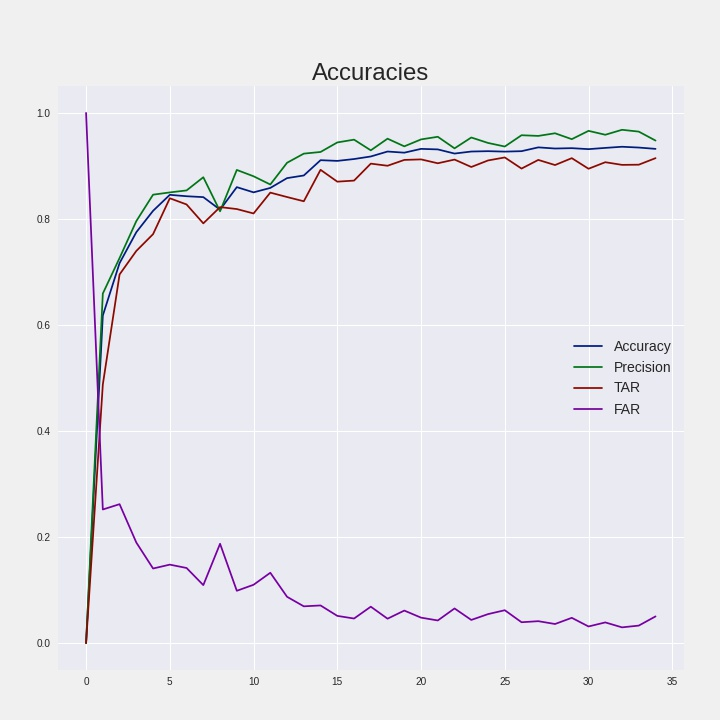
\includegraphics[clip=true,width=\textwidth, height=6cm]{LFWfinal_acc.jpeg}
    \caption{Learning Curves}
    \label{fig:acc}
    \end{minipage}
\end{figure*}

\ptitle{Biometrics} There are four possible outcomes from a binary classifier. If the outcome from a prediction is \textit{p} and the actual value is also \textit{p}, then it is called a \textit{true positive} (TP); however if the actual value is \textit{n} then it is said to be a \textit{false positive} (FP). Conversely, a \textit{true negative} (TN) has occurred when both the prediction outcome and the actual value are \textit{n}, and \textit{false negative} (FN) is when the prediction outcome is \textit{n} while the actual value is \textit{p}. The performance of biometric systems is expressed on the basis of the following error rates:
\begin{raggedright}
\begin{enumerate}
\item \textit{Accuracy} $\displaystyle{ = \frac{\text{TP + TN}}{\text{TP+FP+FN+TN}}}$
\item \textit{True Acceptance Rate} also known as \textit{sensitivity} or \textit{recall}
\begin{equation}
\nonumber \displaystyle{\text{TAR} = \frac{\text{TP}}{\text{TP+TN}} = 1-\text{FRR}}
\end{equation}
\item \textit{False Acceptance Rate (FAR)}
\begin{equation}
\nonumber \displaystyle{\text{FAR} = \frac{\text{FP}}{\text{FP+TN}} = 1-\text{TAR}}
\end{equation}
\item \textit{True Rejection Rate (TRR)} also known as \textit{specificity}
\item \textit{False Rejection Rate (FRR)}
\end{enumerate}
\end{raggedright}
The ROC curve Fig. \ref{fig:roclfw} is useful to understand the trade-off in TAR and FAR for different thresholds. We use Youden’s J statistic to determine the best threshold for the classification. 
\begin{eqnarray}
\nonumber {\displaystyle J={\text{sensitivity}}+{\text{specificity}}-1} \\
\nonumber {\displaystyle J={\frac {\text{TP}}{{\text{TP}}+{\text{FN}}}}+{\frac {\text{TN}}{{\text{TN}}+{\text{FP}}}}-1}
\end{eqnarray}

\section{\label{sec:IvLabs}IvLabs}
\ptitle{Dataset Information} A custom dataset of faces of Lab members. We used the MTCNN \cite{Zhang_2016} framework to detect and align faces provided by \textcite{davidfacenet} to extract the dataset. The images of the members were taken from and can be viewed at \url{https://www.ivlabs.in/core-coordinators.html}. For face-detection on raspberry-pi, we used MobiFace \cite{https://doi.org/10.48550/arxiv.1811.11080}

\ptitle{Outcome} We implemented both FaceNet \cite{Schroff_2015} and ArcFace \cite{Deng_2021} frameworks for this dataset, using transfer learning. We used pre-trained weights on ImageNet for the ResNet18 backbone and trained on the LFW trainset. We fined tuned on IvLabs' face dataset as a classification task by freezing the weights of the backbone and adding a softmax classifier head. We used SGD with a momentum of 0.9, a learning rate of 0.0005, and a one-cycle scheduler from [Paper] for 100 epochs and max. value of the learning rate as 0.005. The predictions are shown in Fig. \ref{fig:ivpreds}

\onecolumngrid
\begin{center}
\begin{figure}[b!]
\begin{center}
    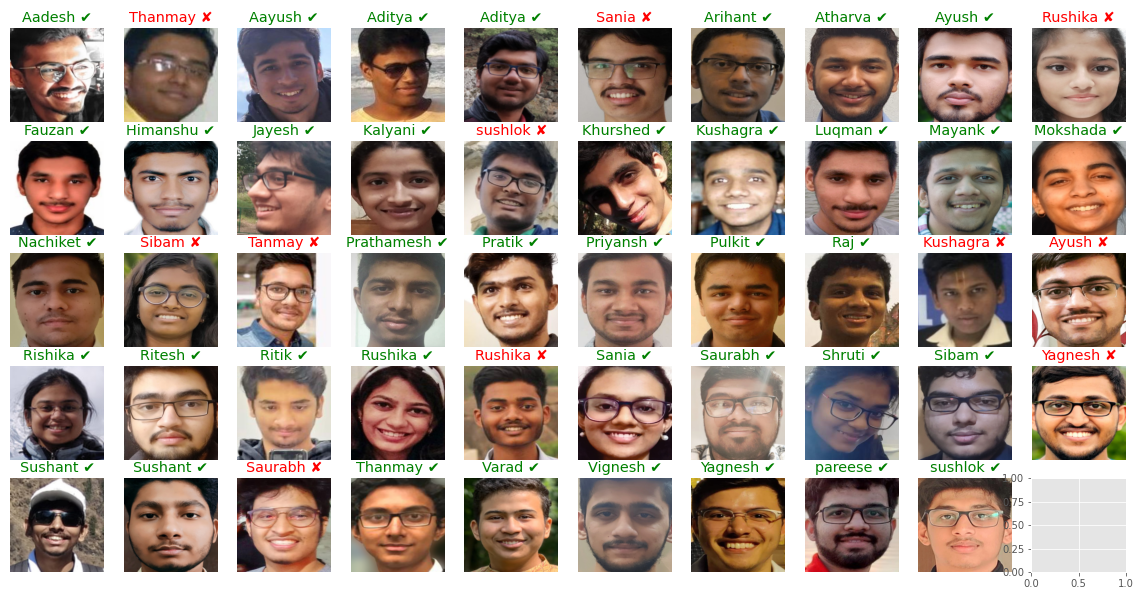
\includegraphics[clip=true,width=\columnwidth]{IvPreds.png}
    \caption{Results on IvLabs' Face Dataset} 
     \label{fig:ivpreds}
\end{center}
\end{figure}
\end{center}
\twocolumngrid

% ---END---

% \begin{itemize}[label=$\Box$]
% \item Check math \& symbolic formatting, as in Table \ref{tab:mathformat}.
% \begin{table}[h!]
%   \begin{center}
%     \caption{Formatting mathematical symbols.}
%     \label{tab:mathformat}
%     \begin{tabular}{c|c} % <-- Alignments: l for left, c for center, and r for right, with vertical lines in between
%       \hline
%       \textbf{Incorrect} & \textbf{Correct} \\
%       \hline \hline
%       $cos \theta$ & $\cos \theta$ \\
%       $T_{sample}$ & $T_\mathrm{sample}$ \\
%       V$_{rms}$, V (rms) & $V_\mathrm{rms}$ \\
%       $E_\mathrm{x}$, x direction & $E_x$, $x$ direction \\
%       $\vec{B_\mathrm{app}}$ & $\vec{B}_\mathrm{app}$ \\
%       $Sb_2Te_3$, Sb2Te3 & Sb$_2$Te$_3$ \\
%       Sb$_{2-\mathrm{x}}$V$_\mathrm{x}$Te$_3$ & Sb$_{2-x}$V$_x$Te$_3$ \\
%       dI/dV & $dI/dV$ \\
%       $B = 5 T$, B=5T & $B=5$ T \\
%       x direction, X direction & $x$ direction \\
%       1st, $1^{st}$, 2nd, $2^{nd}$ & 1$^\mathrm{st}$, 2$^{\mathrm{nd}}$ \\
%       \hline
%     \end{tabular}
%   \end{center}
% \end{table}
% \item Use {\tt \textbackslash label\{tab:name\}} and {\tt \textbackslash ref\{tab:name\}} to refer to tables.
% \item Check hyphenation. Sometimes \LaTeX\ likes to divide a single letter off the beginning or end of a word, for line wrapping. The default settings for \LaTeX's hyphenation of English-language words are {\tt \textbackslash righthyphenmin=3} and {\tt \textbackslash lefthyphenmin=2}, but apparently they can be mysteriously reset to allow single dangling letters.
% \item Check spacing. When a period falls in the middle of a sentence, use a {\tt \textbackslash} (backslash) to prevent \LaTeX\ from thinking it's the end of the sentence and thus adding extra space, as shown in Table \ref{tab:spacing}. If you want to prevent a linebreak, you can use {\tt \textasciitilde} instead of {\tt \textbackslash}.
% \begin{table}[h!]
%   \begin{center}
%     \caption{Spacing.}
%     \label{tab:spacing}
%     \begin{tabular}{l|c|c} % <-- Alignments: l for left, c for center, and r for right, with vertical lines in between
%       \hline
%        & \LaTeX & Output \\
%       \hline \hline
%       Incorrect & {\tt e.g.\ incorrect} & e.g. \ incorrect \\
%       Incorrect & {\tt Fig.\ 2} & Fig. \ 2 \\
%       Correct & {\tt e.g.\textbackslash\ correct} & e.g.\ correct \\
%       Correct & {\tt Fig.\textbackslash\ 2} & Fig.\ 2 \\
%       Correct & {\tt Fig.\textasciitilde 2} & Fig.~2 \\
%       \hline
%     \end{tabular}
%   \end{center}
% \end{table}

% \item Number all equations. But do not separately number each line of a single multi-line equation.
% \item Use {\tt \textbackslash label\{eqn:name\}} and {\tt \textbackslash ref\{eqn:name\}} to refer to equations.
% \item If the equation is mid-paragraph, use {\tt \textbackslash noindent} at the beginning of the first line following the equation.
% \end{itemize}
% \vspace{2mm}

% \ptitle{Equations} Here is an improperly-labeled equation in the middle of a paragraph.
% % Simple equation with no number; this is not a good idea!
% \[
% 1+1=2
% \]
% \noindent Use {\tt \textbackslash noindent} to prevent indentation mid-paragraph. Here is a more interesting example of a properly labeled equation: the Pythagorean theorem relates the 3 sides of a right triangle according to Eqn.\ \ref{eqn:Pythagoras},
% % Here is a proper equation with a number and a label, so that it can be referenced later.
% \begin{equation}
% a^2+b^2=c^2 \,.
% \label{eqn:Pythagoras}
% \end{equation}
% \noindent Eqn.\ \ref{eqn:diagonal} shows one more example of a multi-line equation extending the Pythagorean theorem to find the diagonal $d$ of a rectangular prism of sides $a=3$, $b=4$, and $c=12$.
% \begin{eqnarray}
% \label{eqn:diagonal}
% \nonumber d & = & \sqrt{a^2 + b^2 + c^2} \\
% & = & \sqrt{3^2+4^2+12^2} = 13
% \end{eqnarray}

% \section{\label{sec:Style}Style \& Grammar}

% \begin{itemize}[label=$\Box$]
% \item Use the active voice. If you use the passive voice, it is very hard to tell the difference between what you personally worked hard to do in your experiment, vs.\ what you are citing as a prior result. Use of the active voice is an important component of ethical credit attribution.
% \item Avoid pronouns if at all possible (e.g.\ not ``that'' but ``that voltage signal'').
% % \item The word ``this'' must always be followed by a noun, so that its reference is explicit. Not: This is a fast reaction; This leads us to conclude But: This reaction is fast; This observation leads us to conclude
% \item Use adjectives if there is any doubt (e.g.\ not ``the modulation'' but ``the $z$ modulation'').
% \item Use parallel list structure: ensure that each item in a list (or an ``and'' statement) is the same part of speech and the same category of thing. Not ``we demonstrated apples and the observation of bananas'' but ``we demonstrated apples and bananas''.
% % \item Describe experimental results uniformly in the past tense (e.g.\ not ``Landau levels appear when $B$ is applied'' but ``Landau levels appeared when $B$ was applied'').
% % \item Complete all comparisons (e.g.\ not ``The signal was stronger at 2 Kelvin'' but ``The signal was stronger at 2 Kelvin than at 4 Kelvin'').
% \item Define all acronyms and symbols at first use; then use the acronym consistently from that point on.
% \item Don’t capitalize the words you are about to turn into an acronym. Not``Scanning Tunneling Microscopy (STM)'' but``scanning tunneling microscopy (STM)''. Not ``liquid Mercury (Hg)'' but ``liquid mercury (Hg)''.
% \item Do not use the word ``significantly'' unless you mean it in the true statistical sense and are prepared to back it up quantitatively.
% \item Do not use the word ``successfully'' -- just say what you did and let it speak for itself.
% %\item Journals also typically don't like the words ``new'' or ``novel''. It can be ok to use these words sparingly in a first submission, to catch the editor's or referee's attention, but these words should not be overused.
% \item Remove redundancy, including redundancy between main text and figure captions. When in doubt, the information probably belongs in the caption but not the main text.
% \item Check that all equations are dimensionally correct.
% \item For each equation, define all symbols in a previous equation or in the surrounding text.
% \item Report each quantity consistently throughout the text (e.g.\ don't exaggerate a quantity in one place, give an exact version of the same quantity in another place, and round to the nearest 100 in a third place).
% \item Check that all numbers have units.
% \item Use reasonable significant figures, report errors where appropriate, and clearly explain the method of error determination \cite{WitkovZengel2019}.
% \item When in doubt, check examples (e.g.\ if you wonder whether acronyms are appropriate in the abstract, check a few recent published examples in your target journal).
% \item ``Only'' can be an adjective or an adverb, so its meaning can be ambiguous. It should be placed immediately before the noun, adjective, or verb that it is modifying. For example ``I only bought groceries at the store'' means I didn't dance or sing at the store, I only bought. But ``I bought only groceries at the store'' means I didn't buy party balloons at the store.
% \item ``Its'' is possessive;\\ ``it's'' is a contraction of ``it'' and ``is''.
% \item ``fewer'' describes discrete items, whereas ``less'' describes continuous substances \cite{FewerLess}.
% \item ``which'' vs.\ ``that'': If the sentence doesn't need the clause that the word in question is connecting, use which. If it does, use that \cite{WhichThat}.
% \item ``affect'' vs.\ ``effect'': Each word can be an adjective or a noun, with very different meanings \cite{AffectEffect}.
% \item See additional tips from Prof.\ Margo Seltzer \cite{SeltzerPetPeeves}.
% \end{itemize}

% \section{\label{sec:Figures}Figures}

% \ptitle{Figure style} It is worth taking 2-3 hours to read the definitive guide to ``The Visual Display of Quantitative Information'' by Edward Tufte \cite{TufteVisualDisplay2001}. Tufte defines several metrics for figure optimization:

% \vspace{2mm}
% \noindent $\displaystyle{\text{Data-ink ratio} = \frac{\text{data-ink}}{\text{total ink used to print the graphic}}}$
% \vspace{-1mm}
% \begin{eqnarray}
% \nonumber & = 1.0 - & \text{fraction of a graphic that can be} \\[-2pt]
% \nonumber & & \text{erased without loss of data-information}
% \end{eqnarray}

% \vspace{1mm}
% \noindent $\displaystyle{\text{Data density} = \frac{\text{number of entries in a data matrix}}{\text{area of data graphic}}}$
% \vspace{3mm}

% \noindent A clear and visually pleasing figure should:
% \begin{itemize}[label=$\Box$]
% \item Maximize data-ink ratio.
% \item Maximize data density.
% \item Avoid ``chart-junk'', i.e.\ hatching patterns that interact with the natural motion of the eye to promote the distracting perception of vibration in a static graphic.
% \item Avoid excessive colors.
% \item Avoid red-green combinations (5-10\% of people are red-green colorblind! \cite{CrameriNatCom2020})
% \item Use concise but clear words (not inscrutable abbreviations) directly on the graphic, so the reader doesn't have to dig through a lengthy caption or text to understand the components of the figure.
% \item Orient words horizontally whenever possible.
% \end{itemize}
% \vspace{3mm}

% \ptitle{Use vector format figures} Figures should typically be made in Python, Adobe Illustrator, or other program that allows vector format export, so that all fonts, arrows, etc.\ will scale cleanly when zoomed. Most journals prefer to stay away from Microsoft Powerpoint (although it can be exported to eps or pdf) because the fonts are often not transcribed correctly in publication format. A bigger problem with Microsoft is that it does not faithfully reproduce the pixelation of data images. Microscope images are acquired with a specific pixel resolution, and that pixelation should be honestly communicated to the reader without interpolation. Fig.\ \ref{fig:pixels} illustrates this point.

% \begin{figure}[h]
%     \includegraphics[clip=true,width=\columnwidth]{pixel-compare}
%     \caption{Comparison between blurry pixels (dishonest interpolation occurs when the image is processed in Microsoft Powerpoint) vs.\ clean pixels (honest representation is preserved when the image is processed in Python and Adobe Illustrator). MFM images of vortices in NdFeAsO$_{1-x}$F$_x$ \cite{ZhangPRB2015}.}
%      \label{fig:pixels}
% \end{figure}

% \ptitle{Figure file size} Note that faithful representation of images in vector format usually also results in a smaller figures size. This can be important, because some journals and preprint servers have strict size limits on components of a submitted manuscript.

% \ptitle{Figure font size} All figure fonts should be at least size \minfont\ in the final publication figure \cite{deBivort}. Note also that san-serif fonts are preferred by most journals (e.g. Arial, Helvetica). To achieve the appropriate font size, please start by measuring the desired final figure size (e.g.\ one or two column width) in the desired journal. Then make a box in Adobe Illustrator (or other program) of exactly the final size, and build your figure within it, using no fonts smaller than size \minfont. Although some journals do prefer that you initially submit your figure at full-page size, you can easily scale up your figure for this purpose. But if you start with a page-size figure and arbitrary font sizes, it becomes harder to later scale it down while maintaining adequate font size.

% \vspace{2mm}
% \noindent \textbf{Figure checklist:}
% \begin{itemize}[label=$\Box$]
% \item Use consistent font, at least size \minfont.
% \item Label all axes, with units.
% \item Each plot should have a legend that describes {\em all} symbols and lines.
% \item Each image (or set of same-scale images) should have an accurate length scalebar, with numerical label. (Note that some journals discourage or ``forbid'' superimposing the numerical length on the image. But our goal is clarity: we want the reader to understand the image at a glance, without digging through a lengthy caption to find the necessary number. Journals will generally accept this argument for keeping the number on the image.)
% \item Each image (or set of same-palette images) should have a colorbar. The colorbar should be labeled with numerical values and units if possible.
% %\item If possible, choose colors that will print well in grayscale. But this is no longer a high priority, since most people read online, or have access to color printers.
% \item If using a waterfall plot to display a set of spectra: clearly state the offset of the waterfall plot, or use small horizontal lines to denote the true zero reference for each individual spectrum.
% \item The caption should describes all figure sub-parts, in order. Each and every mark on the figure should be described; there should be no mysterious unexplained arrows or other features.
% \item If any analysis has been performed (i.e.\ if it's not raw data), then all analysis steps should be clearly divulged, usually in the caption (rather than main text).
% \item Clearly explain the origin of all error bars, usually in the caption (rather than main text).
% \item For STM images: give setup conditions in the caption ($V_\mathrm{sample}=100$ mV; $R_J=1$ G$\Omega$).
% \item For STM spectra: give sample bias modulation in the caption ($V_\mathrm{rms}=2$ mV).
% \item For all data: clarify temperature and field conditions in the caption.
% \item Appropriately cite all copied figures or data, in the caption of the figure.
% \item Use {\tt \textbackslash label\{fig:name\}} within the caption, and use {\tt \textbackslash ref\{fig:name\}} in the paper to refer to it.

% \end{itemize}

% \section{\label{sec:References}References}

% \noindent Referencing should be done using BibTeX.
% \begin{itemize}[label=$\Box$]

% \item Consistently use reference tags that will be easily recognizable and editable from the tex file, e.g. {\tt AuthorJournalYear}. Suppose you will be citing
% Huang {\it et al}, Nano.\ Lett.\ 16, 4224 (2016) \cite{HuangNanoLett2016} and
% Huang {\it et al}, Phys.\ Rev.\ B 93, 125129 (2016) \cite{HuangPRB2016}.
% Instead of {\tt Huang2016a} and {\tt Huang2016b}, use {\tt HuangNanoLett2016} and {\tt HuangPRB2016}. (Note: You can make these bib tags within Mendeley.)

% \item Spend 5 minutes to use find-replace with regular expressions to delete the abstracts, keywords, and other useless information from your bib file, to make it easier to read.
% \item Alphabetize the bib entries by author last name, so that it will be easy to notice if there are duplicates. (Note: Mendeley can automatically export them in alphabetical order.)
% \item The hyperlink should be generated from the doi, so make sure every bib entry has a valid doi. You should delete the URL field (unless you are specifically citing a website), because it may contain a non-general URL such as \url{https://journals-aps-org.ezp-prod1.hul.harvard.edu/prb/abstract/10.1103/PhysRevB.93.125129}.
% \item Check the \LaTeX\ formatting of any special characters in the author's names, e.g. {\tt S\textbackslash\textquotesingle\{a\}nchez}
% \item Check the \LaTeX\ formatting in the titles. You need to use extra \{\} around any letters that should be capitalized, e.g.\ {\tt title = \{Quantum Anomalous \{H\}all Effect\} }
% \item Chemical formulas should also be enclosed in \{\} so element abbreviations will be capitalized, e.g.\ {\tt title = \{Experiments on \{Bi\$\_2\$Se\$\_3\$\}\}}. Don't use excessively complicated formatting for chemicals. Just put the subscripts in \$\$.
% \item Use {\tt longbibliography} in the documentclass at the top of the tex file, so that the title of each paper appears in the references.
% \item For most citations, you can just use {\tt \textbackslash cite\{AuthorJournalYear\}}, e.g.\ Jeehoon used conducting force microscopy to measure a metal-insulator transition \cite{KimAPL2010}. But if you're using a superscript citation style, and the citation comes directly after a number or chemical formula, use {\tt Ref.\textbackslash\ \textbackslash onlinecite\{AuthorJournalYear\}} instead to avoid confusion, e.g.\ Jessie measured the pinning force on vortices in NdFeAsO$_{1-x}$F$_x$ (Ref.\ \onlinecite{ZhangPRB2015}).
% \item In the compiled PDF, check all the references carefully to make sure they have correctly formatted authors, titles, and hyperlinks.
% \end{itemize}

% \section{\label{sec:Integrity}Professional Integrity Checklist}

% \begin{itemize}[label=$\Box$]
% \item Authorship -- are all major contributors and collaborators included? See the American Physical Society guidelines for authorship \cite{APSauthor}.

% \item Plagiarism -- have you been careful to distinguish between your own work and ideas, as opposed to those of others?

% \item Citations -- have you properly cited prior work, and references that you used?

% \item Data Integrity -- have you clearly described the data analysis methods, and justified any data points that were excluded?

% \item Image Processing -- have you clearly described any processing that was applied to images?

% \item Acknowledgments -- have you given appropriate credit and thanks to collaborators and other individuals or organizations who deserve recognition?

% \item Clarity of collaborative structure -- if this is a joint effort, have you identified people who you worked with on this project? Acknowledgments should clearly state who did which parts of the experiment \& analysis, and who wrote the paper.

% \item Conflicts of Interest -- do you have any conflicts of interest where you or someone close to you stands to gain, financially or otherwise, from this work?
% \end{itemize}

% \section{\label{sec:Conclusion}Final Checklist}

% \begin{itemize}[label=$\Box$]
% \item Think critically about all of your own claims {\em and} about all of the claims made by your coauthors. If you do not understand something that your coauthor has written in the draft, push back until you do understand, then suggest an alternative phrasing to clarify the manuscript or figure.
% \end{itemize}

% \begin{acknowledgments}
% We acknowledge advice from Jessie Zhang and Harry Pirie to produce Fig.\ \ref{fig:pixels}. We also acknowledge a generation of students who have made all of the errors that led to these checklists.
% \end{acknowledgments}

% \appendix

% \section{\label{app:Mendeley}Mendeley}

% Mendeley provides a convenient (although not 100\% bug-free) database structure for storing, sorting, and annotating the papers you read. Mendeley also provides an export function to automatically create your bib file. Here are some tips to use Mendeley most effectively.
% \begin{enumerate}
% \item Download Mendeley: \url{http://www.mendeley.com/}\\ Launch it on your desktop.
% \item Set Mendeley options: Make sure your Mendeley database is set correctly to include the DOI (digital object identifier) field. Go to Tools $\rightarrow$ Options $\rightarrow$ Document Details. Scroll down and make sure the DOI box is checked.
% \item Import paper: In the upper left corner of Mendeley Desktop, click the drop-down menu for ``Add'' and select the bottom option ``Add Entry Manually''. In the dialog box that pops up, scroll down until you find the DOI field. Paste the DOI into the field, and click the little magnifying glass icon to the right of the field. This will auto-populate all of the relevant paper information such as author names, title, etc., without risk of typos due to manual copying.\\
%     \textit{Note 1:} Mendeley also allows you to import directly from a PDF file, and it tries to pull all of the meta-data from the PDF, but the process is imperfect. So it's safest to use the DOI for an error-free import.\\
%     \textit{Note 2:} Even if you use the DOI, some journal titles will not import correctly with special characters, so you may need to manually correct.
% \item Add tags: It's useful to add tags to help sort your imported papers. For example, if you are going to be writing a manuscript in 2019 on superconductivity, you might add the tag ``sc19'' to all the relevant papers that you will be citing in your manuscript.
% \item Export bib file: Select all of the references that you want to include, and go to File $\rightarrow$ Export.  Name your file, and it will add a citation key to each paper (e.g.\ Whitesides2004) and automatically export to a bib file.
% \item Resolve redundant citation keys: At this point, you may have several references with the same citation key, e.g.\ Huang2016a and Huang2016b \cite{HuangNanoLett2016, HuangPRB2016}. For your future convenience, you should manually change the redundant citation keys to be more informative, e.g.\ HuangNanoLett2016 and HuangPRB2016. Now re-export the bib file.
% \item Open the bib file in your tex file editor. By default, Mendeley exports all fields, including long ones like the abstract. To reduce clutter in your bib file, and make it easier to debug any errors, it's a good idea to remove the abstracts and other unnecessary fields. For example, in WinEdt go to Search $\rightarrow$ Replace, check the regular expressions box, search for ``{\tt <abstract**\textbackslash\},>},'' and replace it with nothing.
% \end{enumerate}

% \section{\label{app:REVTeX}REVTeX}

% \noindent How to install REVTeX 4-2 on Windows for MikTex:
% \begin{enumerate}
% \item Download REVTeX 4-2:\\ \url{http://authors.aps.org/revtex4/}
% \item Unzip the downloaded folder revtex4-2-tds
% \item If you don't already have one, create a folder C:\textbackslash TeX-local
% \item Copy the four subfolders (bibtex, doc, source, tex) into C:\textbackslash TeX-local
% \item From the start menu, open MikTex 2.9 $\rightarrow$ Maintenance (Admin) $\rightarrow$ Settings
% \item On the root tab, add the path C:\textbackslash TeX-local
% \item On the general tab, click ``Refresh FNDB''
% (You may need to close WinEdt, or whatever is using your MikTex installation, in order to properly ``Refresh FNDB''.)
% \item Download natbib:\\
% \url{http://www.ctan.org/tex-archive/macros/latex/contrib/natbib/}
% \item Unzip natbib.
% \item Open natbib.ins, and run TeX on it (Shift+Ctrl+T in WinEdt)
% \item Open bibentry.ins, and run TeX on it (Shift+Ctrl+T in WinEdt)
% %\item You may also need to get two more packages, i.e.\ download from ctan and run TeX on url.ins and textcase.ins
% \end{enumerate}

% %\newpage % acts like \columbreak for a 2-column doc
% \section{\label{app:vectorfig}Vector Graphics}

% To create vectorized graphics from python, include {\tt rasterized=True} inside the {\tt imshow} command. Unfortunately, this preference doesn't seem to be allowable as a default in any style sheet, so you need to remember to include it it every time. Then save the python figure as a PDF, which ensures that annotations (like scale bars, axis labels, and lines) remain as vector format, but images retain their proper pixelation. For example:

% \begin{minted}[mathescape, linenos]{python}
% fig, ax = subplots(1, 1, figsize=[1.8,1.6])
% ax.imshow(a.Z, cmap=stmpy.cm.blue2, aspect=1,
%   clim=(0,1.4), rasterized=True)
% ... 
% tight_layout(pad=0)
% savefig("topo.pdf")
% \end{minted}

% \noindent Note that some PDF viewers apply their own smoothing to images. For example, MacOS Preview may blur images that look fine in Adobe Illustrator.

\bibliography{Hoffman-example-paper}

\end{document}
